% Page: Confidence intervals
% sources/stat2004/chapters/inf-03-confidence-intervals.qmd
% Twenty independent runs of the known-variance interval
%   Xbar ± z_{0.975} * sigma/sqrt(n),
% drawn with mu = 0 and sigma/sqrt(n) = 1, so the half-width is 1.960.
% The centres are a Normal(0,1) sample (seed 9). Two intervals miss mu.
% The coverage 0.95 is the long-run property of the procedure.
\documentclass[border=6pt]{standalone}
\usepackage[T1]{fontenc}
\usepackage{lmodern}
\usepackage{amsmath,amssymb}
\usepackage{tikz}
\usepackage{pgfplots}
\pgfplotsset{compat=1.18}
\definecolor{ink}{HTML}{1F2430}
\definecolor{statblue}{HTML}{174A7E}
\definecolor{accent}{HTML}{9C4A32}
\definecolor{grey}{HTML}{5E6A75}
\pgfplotsset{
  stat/.style={
    scale only axis,
    axis lines=left,
    axis line style={ink, line width=0.6pt},
    tick style={ink, line width=0.45pt},
    tick label style={font=\small, text=ink},
    label style={font=\small, text=ink},
    title style={font=\small, text=ink, align=center},
    unbounded coords=jump,
    scaled ticks=false,
  },
}
\begin{document}
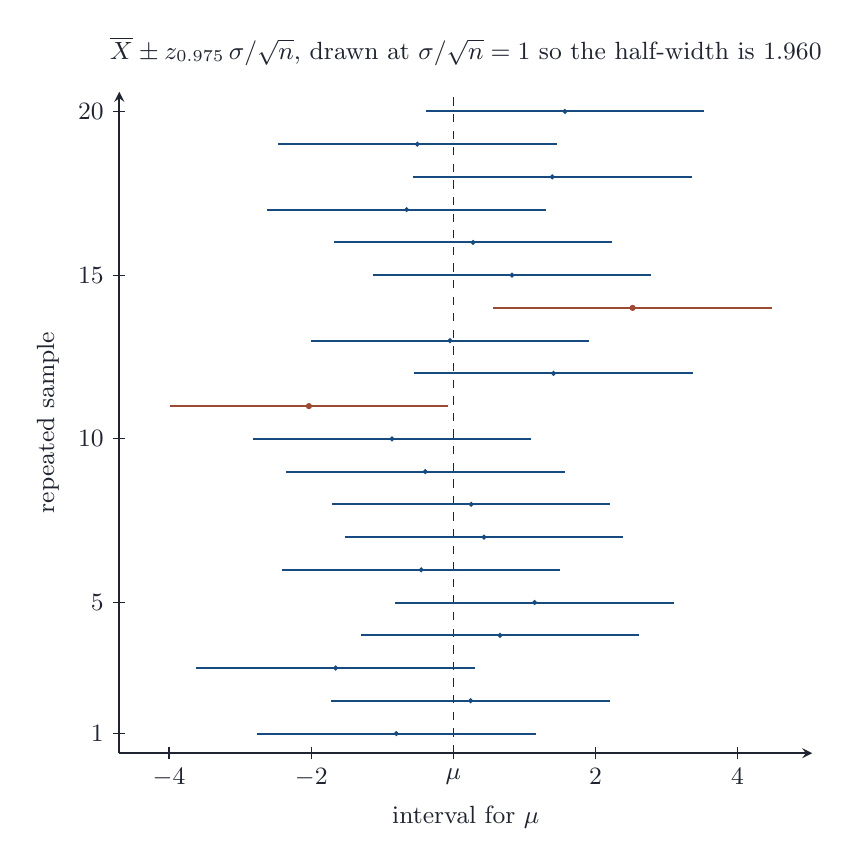
\begin{tikzpicture}
\begin{axis}[
  stat, width=8.8cm, height=8.4cm,
  xmin=-4.7, xmax=5.05, ymin=0.4, ymax=20.6,
  xtick={-4,-2,0,2,4},
  xticklabels={$-4$,$-2$,$\mu$,$2$,$4$},
  ytick={1,5,10,15,20},
  xlabel={interval for $\mu$},
  ylabel={repeated sample},
  title={$\overline{X}\pm z_{0.975}\,\sigma/\sqrt{n}$, drawn at $\sigma/\sqrt{n}=1$ so the half-width is $1.960$},
  clip=false,
]
  \draw[ink, thin, dashed] (axis cs:0,0.4) -- (axis cs:0,20.6);
  \draw[statblue, line width=0.7pt] (axis cs:-2.7628,1) -- (axis cs:1.1572,1);
  \draw[statblue, line width=0.7pt] (axis cs:-1.7171,2) -- (axis cs:2.2028,2);
  \draw[statblue, line width=0.7pt] (axis cs:-3.6163,3) -- (axis cs:0.3037,3);
  \draw[statblue, line width=0.7pt] (axis cs:-1.3039,4) -- (axis cs:2.6161,4);
  \draw[statblue, line width=0.7pt] (axis cs:-0.8165,5) -- (axis cs:3.1035,5);
  \draw[statblue, line width=0.7pt] (axis cs:-2.4126,6) -- (axis cs:1.5074,6);
  \draw[statblue, line width=0.7pt] (axis cs:-1.5295,7) -- (axis cs:2.3905,7);
  \draw[statblue, line width=0.7pt] (axis cs:-1.7091,8) -- (axis cs:2.2109,8);
  \draw[statblue, line width=0.7pt] (axis cs:-2.3544,9) -- (axis cs:1.5656,9);
  \draw[statblue, line width=0.7pt] (axis cs:-2.8224,10) -- (axis cs:1.0976,10);
  \draw[accent, line width=0.95pt] (axis cs:-3.9926,11) -- (axis cs:-0.0726,11);
  \draw[statblue, line width=0.7pt] (axis cs:-0.5496,12) -- (axis cs:3.3704,12);
  \draw[statblue, line width=0.7pt] (axis cs:-2.0076,13) -- (axis cs:1.9124,13);
  \draw[accent, line width=0.95pt] (axis cs:0.5623,14) -- (axis cs:4.4823,14);
  \draw[statblue, line width=0.7pt] (axis cs:-1.1338,15) -- (axis cs:2.7862,15);
  \draw[statblue, line width=0.7pt] (axis cs:-1.6822,16) -- (axis cs:2.2378,16);
  \draw[statblue, line width=0.7pt] (axis cs:-2.6174,17) -- (axis cs:1.3026,17);
  \draw[statblue, line width=0.7pt] (axis cs:-0.5675,18) -- (axis cs:3.3525,18);
  \draw[statblue, line width=0.7pt] (axis cs:-2.4663,19) -- (axis cs:1.4537,19);
  \draw[statblue, line width=0.7pt] (axis cs:-0.3901,20) -- (axis cs:3.5299,20);
  \addplot[only marks, mark=*, mark size=0.7pt, statblue, forget plot] coordinates {
    (-0.8028,1) (0.2429,2) (-1.6563,3) (0.6561,4) (1.1435,5)
    (-0.4526,6) (0.4305,7) (0.2509,8) (-0.3944,9) (-0.8624,10)
    (1.4104,12) (-0.0476,13) (0.8262,15) (0.2778,16)
    (-0.6574,17) (1.3925,18) (-0.5063,19) (1.5699,20)
  };
  \addplot[only marks, mark=*, mark size=0.9pt, accent, forget plot] coordinates {
    (-2.0326,11) (2.5223,14)
  };
\end{axis}
\end{tikzpicture}
\end{document}
